\chapter{Gestión y Planificación del proyecto}



\section{Metodología}

\subsection{Aplicación de la 'metodología' al proyecto}

\section{Gestión de la configuración}
En este apartado se describirá cómo se ha llevado a cabo la gestión de los activos de este proyecto, es decir, el código desarrollado y la documentación generada. Dado que son partes fundamentales del trabajo, atendiendo al análisis de riesgos descrito en la sección \ref{riesgos} y el plan de actuación frente a la pérdida de información, se detalla a continuación la gestión de ambas.

\subsection{Gestión del código}
Para la gestión del código se ha usado un control de versiones a través de Git y Github. Ambas herramientas en conjunto permiten ir creando versiones intermedias del código conforme se va desarrollando y hacer copias de seguridad en la nube. También son muy útiles para proyectos colaborativos, donde varias personas del equipo pueden combinar fácilmente su parte del código desarrollado y revisar el progreso subido hasta el momento.
El procedimiento a seguir en la mayoría de casos es bastante similar. Se creará un repositorio remoto en la plataforma de GitHub con el nombre de \emph{TFG} —o el que uno prefiera— donde se irán almacenando los cambios\footnote{\url{https://github.com/Jesnm01/TFG}}. En la carpeta de trabajo local de nuestra computadora, carpeta que contendrá en mi caso todos los elementos de los que quiera llevar un control, se creará un repositorio local usando Git, que habrá que vincular con el remoto para poder ir sincronizando los cambios. 


\subsection{Gestión de la documentación}
En lo relativo a la documentación, el proceso de gestión será similar ya que también se ha usado GitHub para su control de versiones. Esta se ha redactado en LaTeX usando el servicio online Overleaf. Overleaf cuenta con una opción para sincronizar el proyecto con un repositorio de GitHub, pero es una opción de pago. En su lugar, descargo el proyecto en el repositorio local y desde ahí ya realizo dicha sincronización para subir los cambios en el remoto.

Además, dada la naturaleza del proyecto y de la metodología de desarrollo utilizada, se ha llevado un registro de las reuniones con la tutora que también se ha ido actualizando periódicamente. Este documento pretende recoger los contenidos más relevantes de las reuniones con Rocío: preguntas, comentarios, anotaciones, tareas que hacer, cosas pendientes de una reunión a otra, revisiones, y puntos a mejorar, entre otras cosas.



\section{Gestión de recursos} \label{gestion_recursos}

\subsection{Recursos humanos}
\begin{itemize}
    \item \textbf{Dña. Rocío Celeste Romero Zaliz}, profesora del Departamento de Ciencias de la Computación e Inteligencia Artificial de la Universidad de Granada en calidad de tutora del proyecto. A cargo de la supervisión y guía del alumno durante su desarrollo del trabajo.
    \item \textbf{Jesús Navarro Merino}, estudiante del grado en Ingeniería Informática en la Escuela Técnica Superior de Ingenierías Informática y Telecomunicación.
\end{itemize}


\subsection{Recursos materiales}
Para este proyecto no se han necesitado recursos adicionales, habiéndose usado únicamente los siguientes recursos materiales, ya poseídos por el alumno: 
\begin{itemize}
    \item \textbf{Portátil personal}: Portátil ACER Aspire A515-51G-8907 con un procesador Intel Core i7 8550U 1.8GHz, 20GB de memoria RAM y una arquitectura de 64 bits. Se ha usado durante todo el proyecto, para labores de programación y redacción de la memoria.
    \item \textbf{Pantalla}. Monitor utilizado de apoyo a la pantalla propia del portátil. De la marca AOC, de 24 pulgadas con una resolución de 1920x1080.
\end{itemize}


\subsection{Recursos software} \label{recursos_software}
En esta sección describiré todas aquellas herramientas software empleadas durante la realización del proyecto. Todas y cada una de ellas son herramientas de software libre, gratuitas o disponibles a través de licencias de estudiantado. A continuación se lista el software usado:
\begin{itemize}
    \item \textbf{Sistema operativo}: Windows 10 Home. Aunque por lo general Windows no es gratuito, al estar utilizando la típica licencia OEM que trae preinstalada el ordenador al comprarlo, la considero como tal.
    
    \item \textbf{Visual Studio C++}: es un IDE muy potente de Microsoft orientado a crear aplicaciones .NET y C++ para Windows. Se ha usado su versión gratuita Visual Studio Community 2022. Permite editar, depurar, realizar pruebas de testing, además de tener control de versiones integrado, entre otras cosas. Aquí se ha llevado a cabo todo el desarrollo del código.
    
    \item \textbf{OpenBabel}: Open Babel es una biblioteca de código abierto multiplataforma utilizada en química computacional y ciencias relacionadas para la conversión y manipulación de estructuras químicas en varios formatos. He trabajado con el release 3.1.1 disponible en su repositorio de GitHub oficial\footnote{\url{https://github.com/openbabel/openbabel}}.

    \item \textbf{CMake}: es una herramienta de generación de archivos de compilación que simplifica el proceso de compilación y construcción de proyectos, permitiendo una configuración flexible e independiente de la plataforma. CMake utiliza archivos de configuración llamados CMakeLists.txt para describir la estructura del proyecto y las dependencias necesarias. Se ha usado en su versión 3.25.2 para la compilación y creación de soluciones de OpenBabel.

    \item \textbf{Git}: software de código abierto para el control de versiones de un proyecto.
    \item \textbf{Github}: es una plataforma donde se alojará el código y la documentación del proyecto. Utiliza Git por debajo y es una de las plataformas gratuitas para alojamiento de código mas empleadas a nivel mundial.

    \item \textbf{Google Colab}: es una plataforma en línea gratuita ofrecida por Google que permite a cualquier usuario escribir y ejecutar código Python en el navegador. Es una herramienta basada en la nube que proporciona un entorno de ejecución como si fueran notebooks de Jupyter, es decir, se puede escribir, editar y ejecutar código en bloques/celdas interactivos. Se ha usado durante las etapas iniciales del proyecto para la experimentación con diversas moléculas.
    
    \item \textbf{Zotero}: software de gestión de referencias bibliográficas que permite recopilar, organizar, citar y generar fácilmente una bibliografía en varios estilos de formato estándares según los documentos, páginas webs, artículos o archivos PDF guardados. Facilita la creación de referencias y citas en documentos académicos, ahorrando tiempo y asegurando un uso correcto de las fuentes consultadas.
    
    \item \textbf{Google Meet}: servicio de videoconferencias de Google. Plataforma utilizada para las reuniones con la tutora.

    \item \textbf{Google Drive Sync}: ahora llamada Google Drive para PC, es una aplicación de Google que permite sincronizar los archivos y carpetas de la computadora con la cuenta de Drive. Usado para realizar copias de seguridad —adicionales a lo almacenado en GitHub— de algunos archivos importantes. 

    \item \textbf{Overleaf}: herramienta online para la redacción de documentos en LaTeX usada para la documentación de este proyecto.

    \item \textbf{Correo UGR}: servicio de correo electrónico institucional de la UGR.

    \item \textbf{Microsoft Word}: procesador de textos de Microsoft usado para apuntes personales y documentación en sucio. Disponible a través de la cuenta de Microsoft Office 365 que ofrece la universidad.

    \item \textbf{Microsoft Excel}: utilizado para la creación de algunas tablas y gráficos incluidos en la memoria. Disponible a través de la cuenta de Microsoft Office 365 que ofrece la universidad.

    \item \textbf{Visual Studio Code y LaTeX}: VSCode es un editor de texto, que a través de algunas extensiones, permite editar, compilar y visualizar ficheros LaTeX. Es la alternativa a Overleaf según lo descrito en la sección \ref{riesgos}. 

    
    
\end{itemize}

\section{Gestión de costes}
\textbf{TERMINAR esto cuando vaya acabando el trabajo}

En esta sección se realizará una estimación de los costes asociados al proyecto, atendiendo a los recursos descritos en la Sección \ref{gestion_recursos}. La elaboración de un presupuesto preciso en muchos casos puede suponer un desafío, ya que los proyectos software a menudo están sujetos a cambios y variables imprevistas, pero es una tarea importante para estudiar su viabilidad. 

\subsection{Coste de recursos humanos}
Si actuáramos como una empresa, en un proyecto software al uso existen muchos componentes que tener en cuenta para montar esta sección del presupuesto. Aspectos como el salario de los trabajadores y compensaciones varias, el coste de los procesos de selección y contratación, formación y desarrollo del personal, costes laborales adicionales (seguros, vacaciones, etc), o costes de personal externo (consultores o subcontratistas) entre otras cosas.
Dada la naturaleza de este proyecto, en relación a los gastos asociados a recursos humanos contamos con un equipo de desarrollo formado por una persona que tendrá el papel de Ingeniero Informático. Para calcular el costo de su trabajo, se indica el número total de horas dedicadas y su correspondiente coste.

\textbf{HACER} una estimación segun el horario normal de un trabajador durante todos los dias de X meses. Contrastarlo con las horas reales dedicadas segun clockify.


\subsection{Costes de recursos materiales}

Dado que no se han adquirido expresamente para este proyecto, ya que se poseían con anterioridad, no se valora su precio de compra como tal sino su valor de depreciación. Los productos electrónicos experimentan un proceso llamado depreciación, que conlleva una devaluación gradual a lo largo de su vida útil. Es importante tener esto en cuenta para estimar su valor actual y el coste del recurso. Esta estimación refleja el valor de un activo desde un punto de vista contable.

Al referirnos a la depreciación de un activo a lo largo de su vida útil, no se incluyen situaciones en las que sufra daños debido a accidentes, desastres naturales u otros eventos similares. En cambio, estamos hablando del desgaste del uso cotidiano, así como los impactos derivados de las innovaciones tecnológicas que surgen durante ese período que puedan dejar obsoleto el dispositivo.

Para calcular el valor actual de los activos utilizaré el método de depreciación lineal, que considera un desgaste uniforme durante su uso, mostrando el resultado del gasto anual de depreciación\cite{depreciacion_pcs}. Necesitamos lo primero, hallar el valor residual del activo, es decir, el valor que se estima que tendrá cuando llegue al final de su vida útil. Usaré para los dispositivos electrónicos una vida útil de 8 años. Haré un ejemplo con el coste del portátil.

\begin{equation*}
    \textit{Valor residual} = {\frac{\textit{Coste inicial}}{\textit{Vida util (años)}}} = \frac{689 \EUR{}} {8 \textit{ años}} = 86,125 \EUR{}
\end{equation*}

Con el valor residual estimado, se puede calcular la depreciación lineal anual con la siguiente fórmula.

\begin{equation*}
    \textit{Depreciación} = {\frac{\textit{Coste inicial} - \textit{Valor residual}}{\textit{Vida util (años)}}} = \frac{689\EUR{}-86,125\EUR{}} {8 \textit{ años}} = 75,36 \EUR{}
\end{equation*}

Teniendo estos 2 datos, se puede calcular el valor actual del activo teniendo en cuenta sus años de antigüedad. Se muestran todos los datos relativos a los costes materiales en la Tabla \ref{tabla:costes_materiales}.


\begin{table}[ht]
\small
    \begin{tabular}{lllll}
    \toprule 
    % Al parecer tengo que hacer esto asi tan extraño (meter una tabla de 1 celda dentro de la propia celda para poder meter un salto de linea...)
    \textbf{Recurso} & \textbf{\begin{tabular}[c]{@{}l@{}}Valor\\ inicial (€)\end{tabular}} & \textbf{\begin{tabular}[c]{@{}l@{}}Depreciación\\ anual (€)\end{tabular}} & \textbf{\begin{tabular}[c]{@{}l@{}}Antigüedad\\ (años)\end{tabular}} & \textbf{\begin{tabular}[c]{@{}l@{}}Valor\\ actual (€)\end{tabular}} \\ 
    \midrule
    Portátil personal           & 689 & 75,36 & 5 & 312,2         \\ 
    Pantalla AOC                & ~230 & 25,15 & 2 & 179,69         \\ 
    \midrule
    \multicolumn{4}{r}{\textbf{Total:} } & 491,89 \\
    \bottomrule
\end{tabular}
\caption{Tabla de los costes materiales}
\label{tabla:costes_materiales}
\end{table}

\subsection{Costes software}
Los costes relacionados con los recursos software son nulos. Como indico en el listado de recursos de la Sección \ref{recursos_software}, son herramientas de software libre o utilizadas mediante licencias gratuitas, por lo que no suponen coste alguno en el desarrollo de este proyecto.

\subsection{Otros costes}
Aquí se incluyen todos los demás gastos que han sido necesarios para el desarrollo del proyecto y que no pertenecen a los apartados anteriores. Principalmente son los gastos vinculados a las facturas de la luz e Internet. El coste de la tarifa de Internet contratada es de 40€/mes, que a lo largo de los 5 meses el total asciende a 200€. Para la luz, una estimación posible serían 19,58€, teniendo en cuenta el gasto que suponen los recursos materiales en base a una factura trimestral de 11,80€.

\begin{table}[ht]
    \centering
    \begin{tabular}[t]{lc}
        \toprule
        \textbf{Recursos} & \textbf{Importe (€)}  \\
        \midrule
        Luz         &   19,58   \\
        Internet    &   200      \\
        \bottomrule
    \end{tabular}
    \caption{Tabla de costes adicionales}
    \label{tabla:costes_adicionales}
\end{table}




\subsection{Presupuesto final}
Se presenta por tanto el presupuesto completo asociado al proyecto, dividido en cada una de las secciones tratadas anteriormente. Se ve el desglose en la Tabla \ref{tabla:presupuesto_total}.
\begin{longtable}[c]{lm{3cm}r}
\toprule
\textbf{Detalle}                        && \textbf{Importe} \\
\endfirsthead
%
\endhead
%
% \hline
\endfoot
%
\endlastfoot
%
\midrule
                                        % &                 \\\hline
\textbf{Costes de recursos humanos}     && \textbf{X €} \\
Trabajo autónomo                        && X €          \\
\midrule
\textbf{Costes de recursos materiales}  && \textbf{X €} \\
\multicolumn{2}{c}{Portátil personal:}  & 312,2 €            \\ %Esto para darle un tabulado al elemento
Pantalla de apoyo                       && 179,69 €             \\ 
\midrule
\textbf{Costes de recursos software}    && \textbf{0,00 €}    \\
                                        % & \multicolumn{1}{l}{}    \\
Windows 10                              && 0,00 €             \\
Visual Studio C++                       && 0,00 €             \\
OpenBabel                               && 0,00 €             \\
CMake                                   && 0,00 €             \\
Git                                     && 0,00 €             \\
GitHub                                  && 0,00 €             \\
Google Colab                            && 0,00 €             \\
Zotero                                  && 0,00 €             \\
\multicolumn{1}{r}{Google Meet:}                             && 0,00 €             \\
\multicolumn{1}{c}{Google Drive Sync:}                       && 0,00 €             \\
Overleaf                                && 0,00 €             \\
Correo UGR                              && 0,00 €             \\
Microsoft Word                          && 0,00 €             \\
Microsoft Excel                         && 0,00 €             \\
Visual Studio Code y LaTeX              && 0,00 €             \\
% \midrule
% \textbf{Costes de recursos de comunicación y documentación} & \textbf{0,00 €}  \\
%                                         % & \multicolumn{1}{l}{}                   \\
% Google Meet                             & 0,00 €             \\
% Correo UGR                              & 0,00 €             \\
% Overleaf                                & 0,00 €             \\
% Texmaker                                & 0,00 €             \\
% Visual Paradigm                         & 0,00 €             \\
% Microsoft Powerpoint                    & 0,00 €             \\
\midrule
\textbf{Costes adicionales}             && \textbf{X €}  \\
                                        % & \multicolumn{1}{l}{}                   \\
Internet                                && 40€ x 5 meses = 200€           \\
Factura de la luz                       && 19,58 €            \\
                                        % & \multicolumn{1}{l}{}                   \\
\midrule
  &   \multicolumn{1}{r}{\textbf{Total:}} & \textbf{X €} \\
\bottomrule
\caption{Presupuesto total del proyecto}
\label{tabla:presupuesto_total}
\end{longtable}


\section{Planificación}
Esto quizas deberia ponerlo despues de la metodologia y antes de gestion de la condfiguracion

\section{Análisis de riesgos} \label{riesgos}
El análisis de riesgos desempeña un papel fundamental en la planificación y ejecución exitosa de proyectos. A veces surgen imprevistos que pueden afectar en mayor o menor medida a la correcta evolución de estos. Por ello, la aplicación de este proceso resulta esencial para minimizar la incertidumbre, intentar evitar la aparición de esos riesgos, y en caso de que se materialicen, paliarlos o mitigarlos de manera efectiva mediante unos planes de actuación.

En este aparatado por tanto, se analizarán los riesgos potenciales del proyecto, incluyendo sus causas y el plan de acción para resolverlos o mitigar su impacto al máximo (Figura \ref{tabla:tabla_riesgos}). Además, se realizará una evaluación de la probabilidad de ocurrencia y del impacto asociado a cada riesgo, que se puede ver en la Figura \ref{tabla:riesgos_matriz_probabilidad}. Esto se basa en una matriz con 2 dimensiones: la probabilidad de ocurrencia de un riesgo y el impacto que tendría en el proyecto si se materializa. Se valorarán los riesgos según aspectos técnicos, de recursos humanos o complejidad y naturaleza del proyecto, y preguntas del tipo, ¿qué tan difícil sería recuperarse del riesgo?, ¿cuál es el resultado más negativo que podría originarse como consecuencia? o ¿ha sucedido este riesgo o alguno similar anteriormente?

\begin{figure}
    \centering
    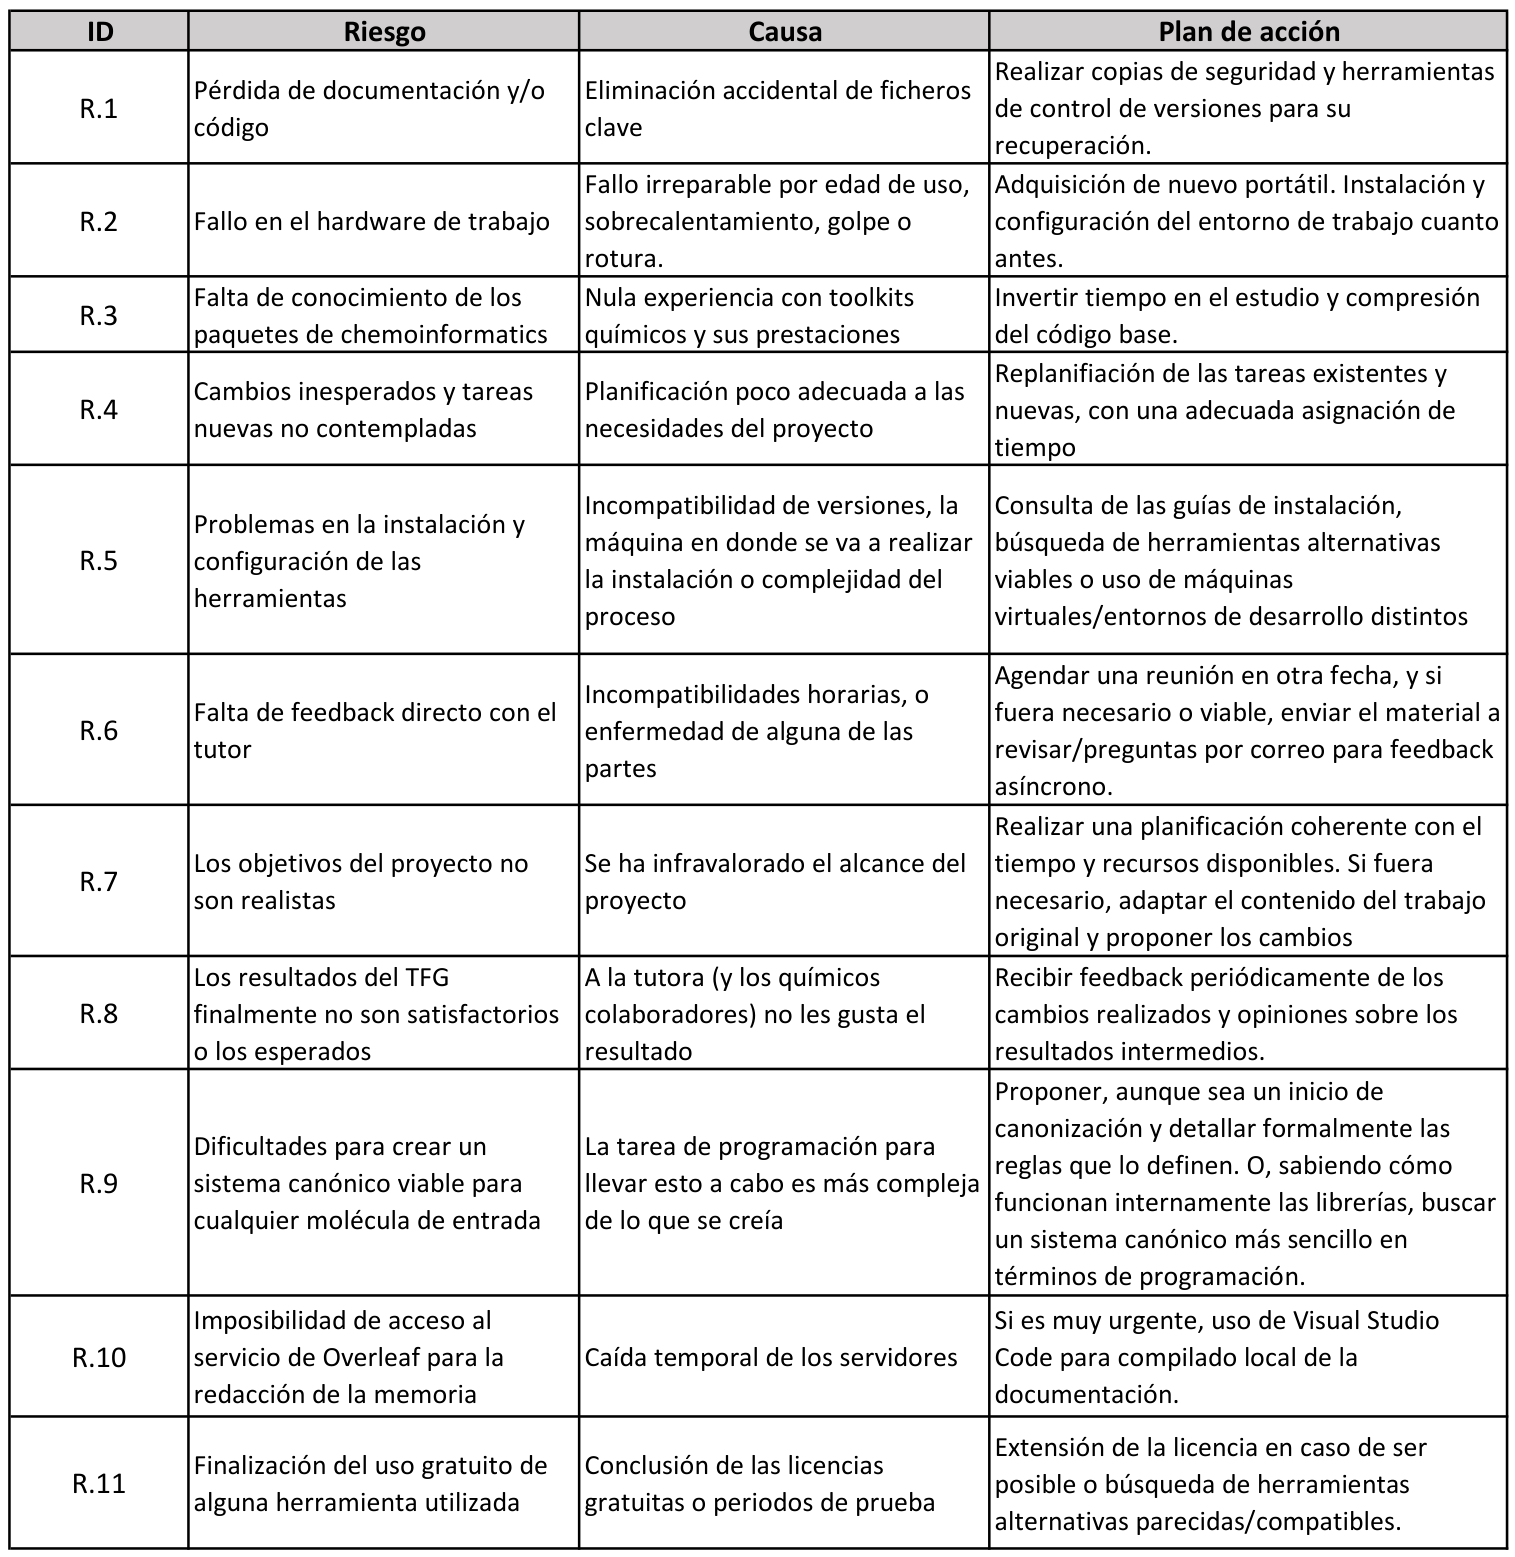
\includegraphics[scale=1]{imagenes/planificacion/riesgos-1_cropped.png}
    \caption{Riesgos del proyecto, causas, y planes de actuación}
    \label{tabla:tabla_riesgos}
\end{figure}

\begin{figure}
    \centering
    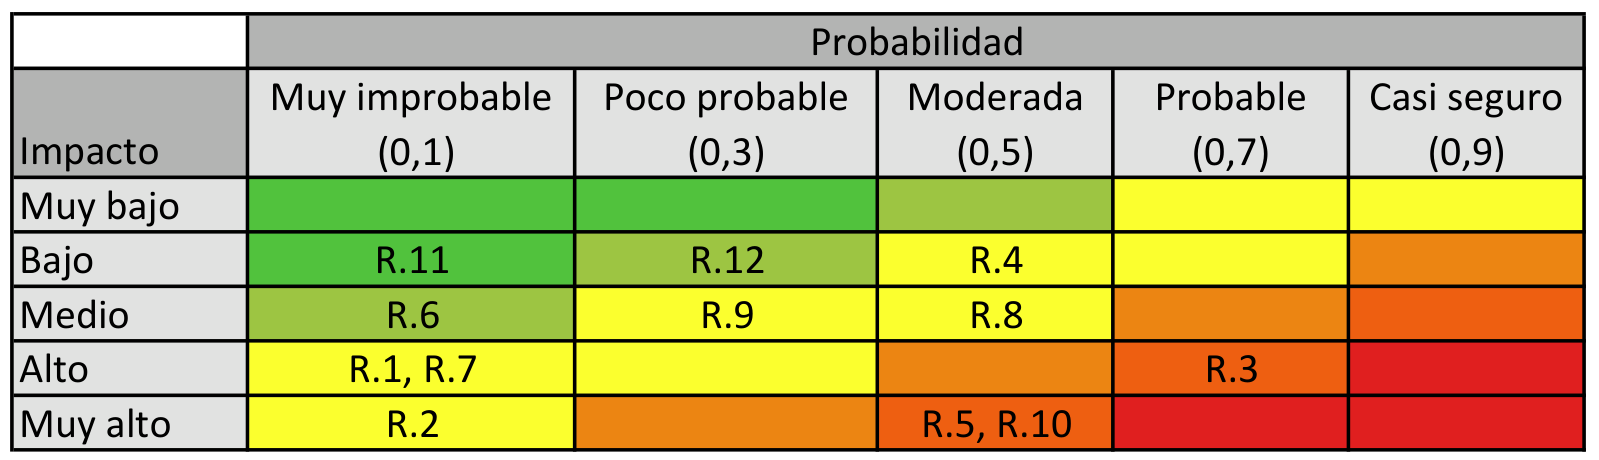
\includegraphics[scale=0.95]{imagenes/planificacion/matriz_riesgos.png}
    \caption{Matriz de probabilidad-impacto de riesgos}
    \label{tabla:riesgos_matriz_probabilidad}
\end{figure}

\subsection{Riesgos materializados}

\textbf{completar esto al final del trabajo, o conforme se vayan ocurriendo}


Los riesgos materializados han estado relacionados principalmente con aspectos técnicos. Primeramente, el R.5. Tuve problemas para instalar OpenBabel en mi máquina por problemas de versiones, por lo que acabé utilizando Google Colab como entorno virtual e instalar ahí algunas librerías y para las primeras experimentaciones con moléculas. Esto tampoco era muy útil a largo plazo puesto que tenía que poder acceder al código fuente para modificarlo, añadir las funcionalidades y compilarlo manualmente para probar los cambios. Por lo que finalmente con ayuda de las guías, se pudo ejecutar localmente. Instantáneamente después, se materializó el riesgo R.3. La falta de conocimiento ante una librería tan grande ya existente retrasó un poco el proceso de modificación del código. 

Finalmente, se consiguieron solventar los riesgos manifestados mediante los planes de actuación descritos en cada uno de ellos.